\subsection{Relations among features}
So far, we only really looked into features separately. This section will now focus on showing how multiple features are related. We will only consider relating TWO features, but the techniques are also applicable to more.

\subsubsection*{Scatter plots}

As a first step to see whether a relation exists, first plot the two features. Examples for typical resulting \textbf{correlations}\sidenote{Correlation} is shown in \ref{fig:2_correlation}.

\begin{figure}[H]
  \begin{subfigure}{0.3\textwidth}
    \centering
    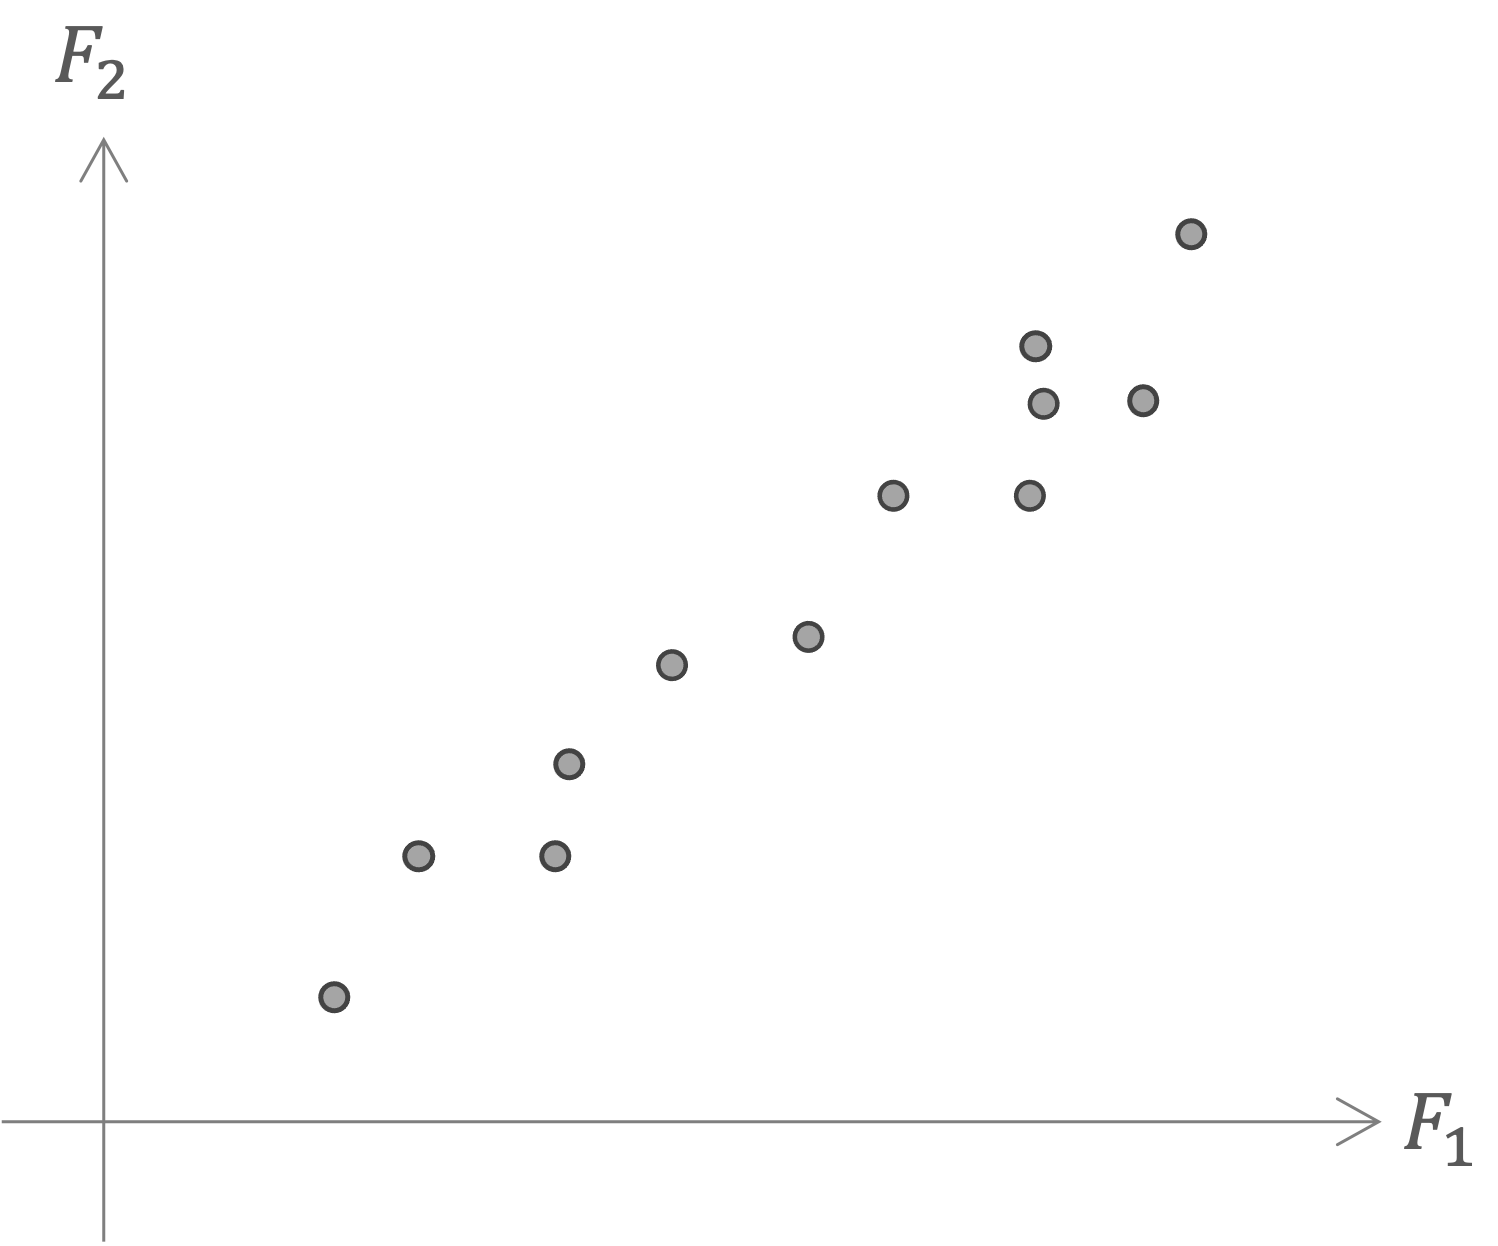
\includegraphics[width=0.9\textwidth]{assets/visualization_and_extraction/feature_relation/scatter_pos_cor.png}
    \subcaption{Positive correlation}
  \end{subfigure}\hspace*{0.025\textwidth}
  \begin{subfigure}{0.3\textwidth}
    \centering
    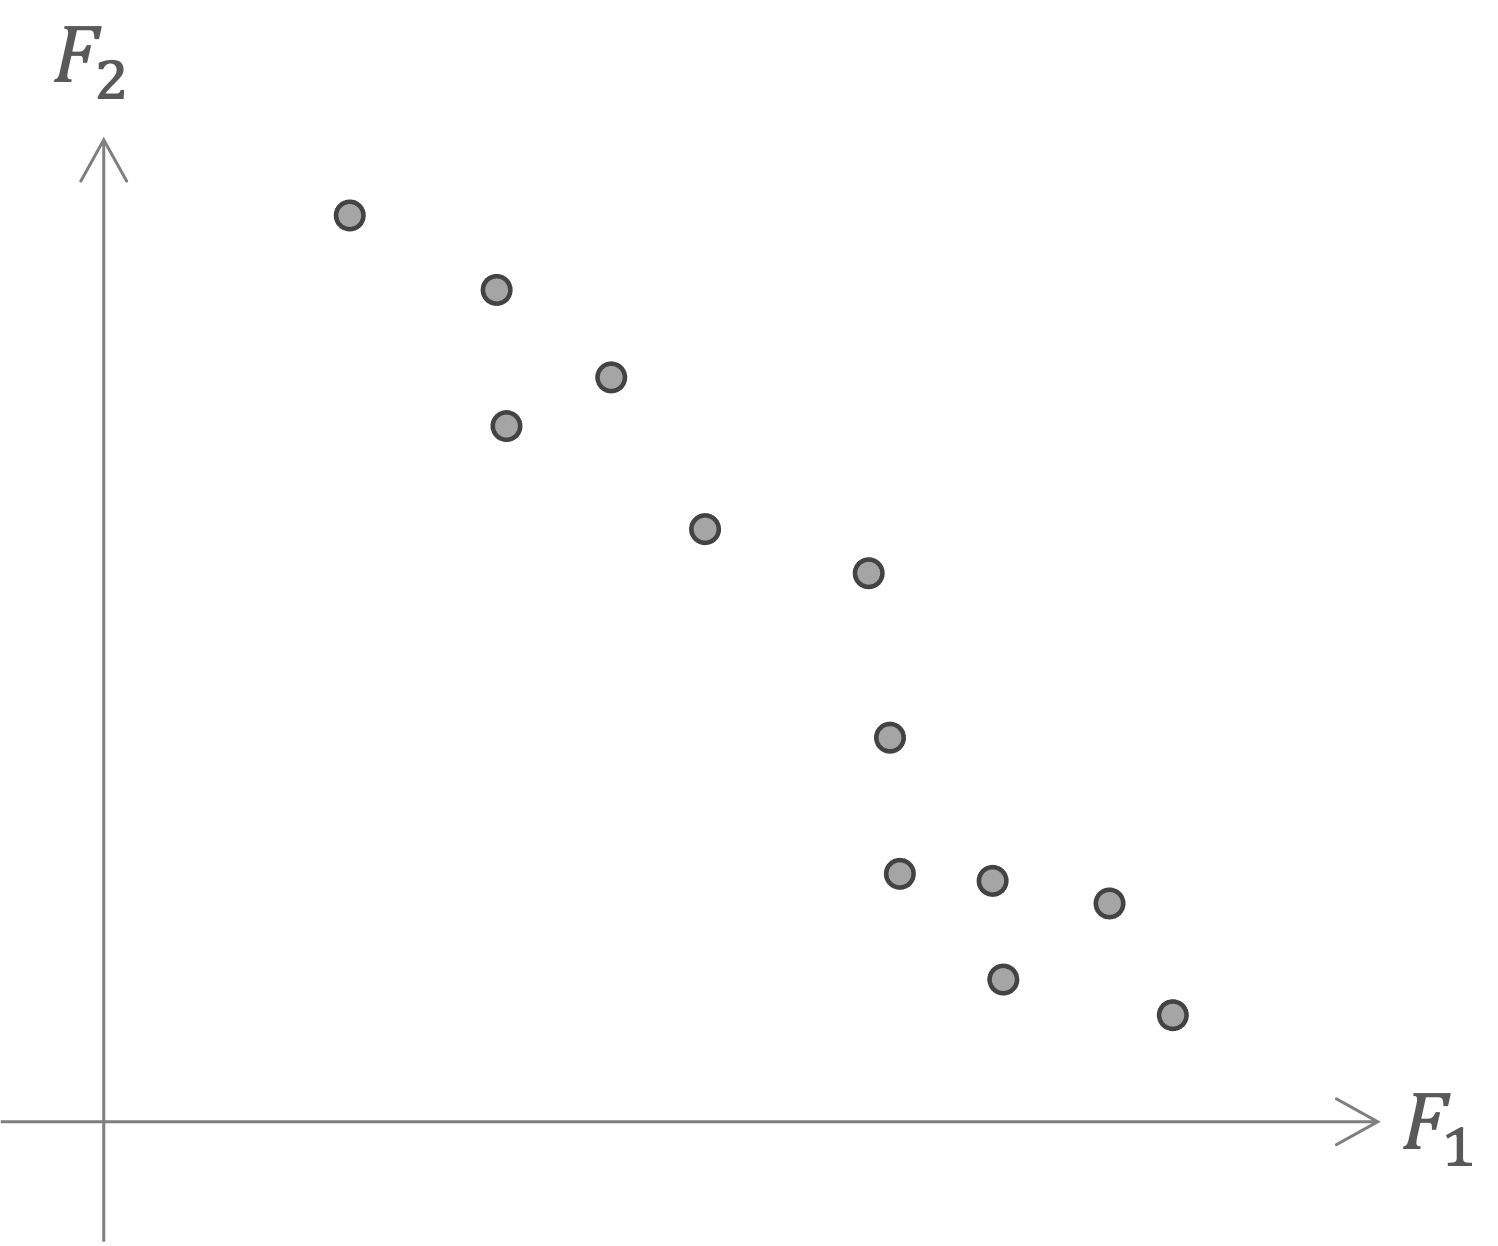
\includegraphics[width=0.9\textwidth]{assets/visualization_and_extraction/feature_relation/scatter_neg_cor.png}
    \subcaption{Negative correlation}
  \end{subfigure}\hspace*{0.025\textwidth}
  \begin{subfigure}{0.3\textwidth}
    \centering
    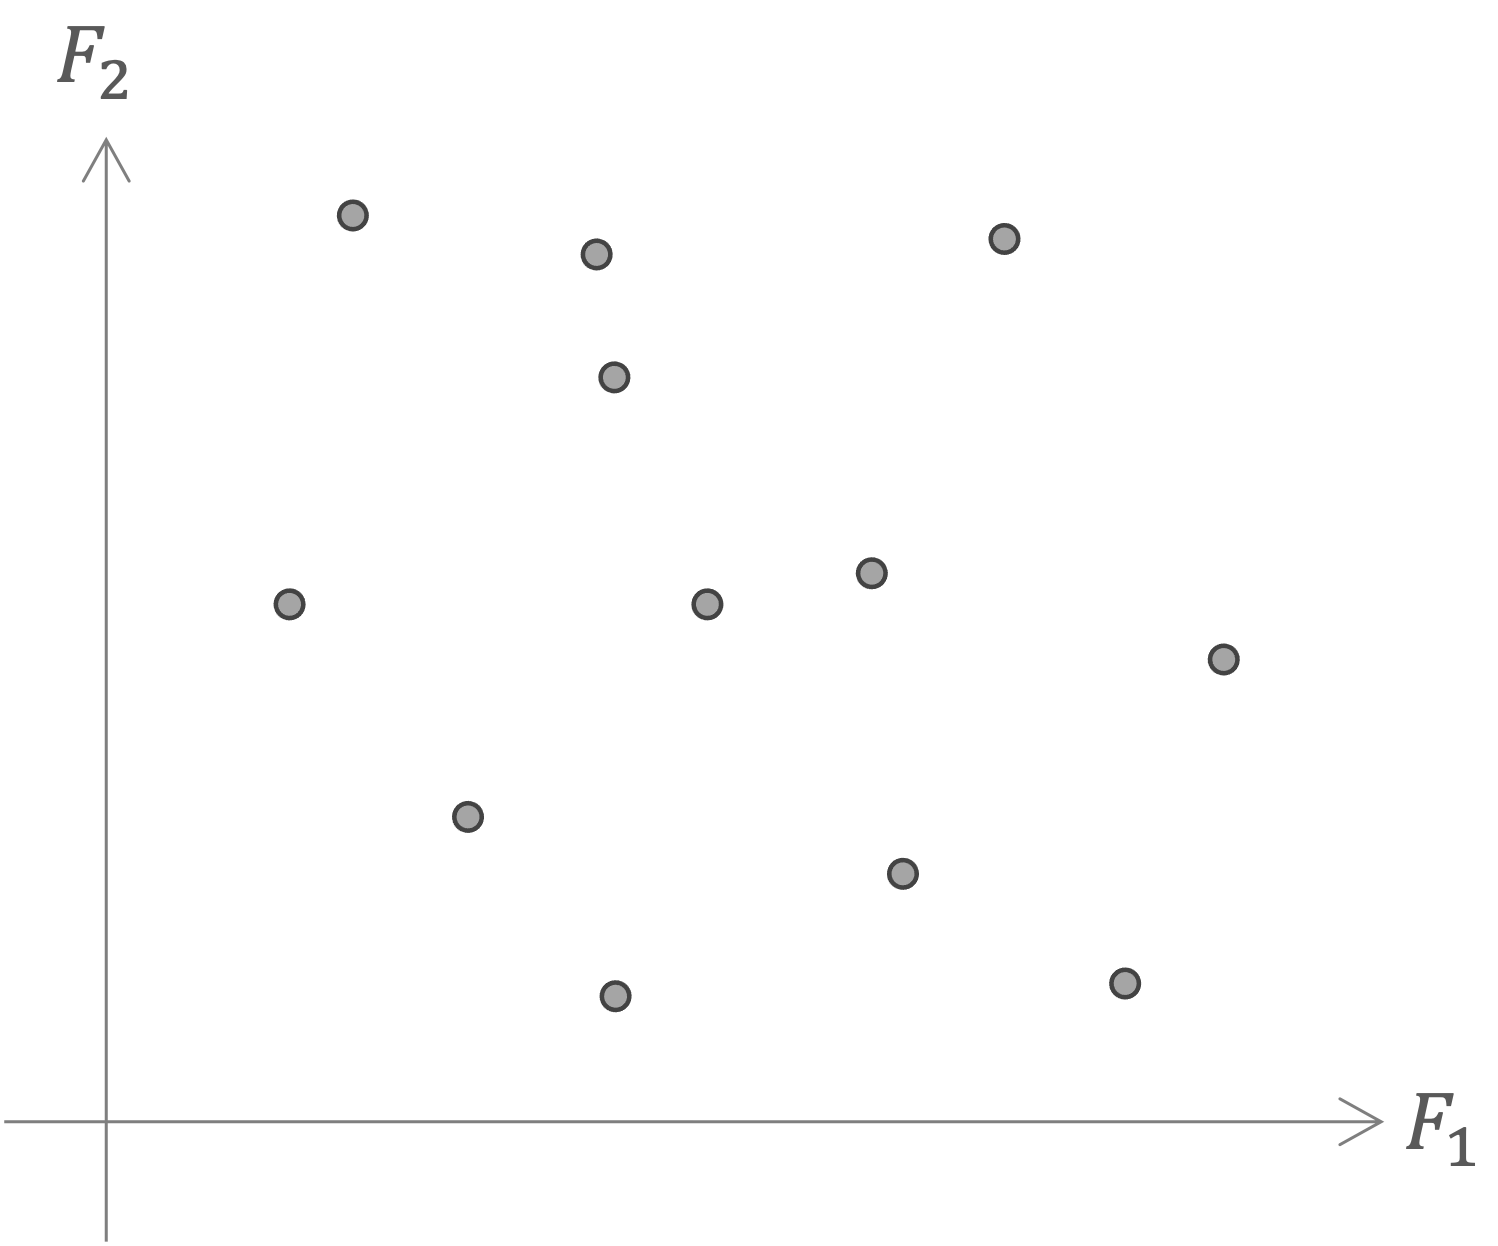
\includegraphics[width=0.9\textwidth]{assets/visualization_and_extraction/feature_relation/scatter_not_cor.png}
    \subcaption{No correlation}
  \end{subfigure}
  \caption{Scatter plots visualizing correlations}
  \label{fig:2_correlation}
\end{figure}

As an example for detecting correlations, we have a data set about basketball players with different features. The raw data will not be included here. Instead, we will directly look at all correlations of the features simultaneously. This is visualized using a \textbf{scatter plot matrix} (SPLOM)\sidenote{SPLOM} as in \ref{fig:2_splom}.

\begin{figure}[h]
  \centering
  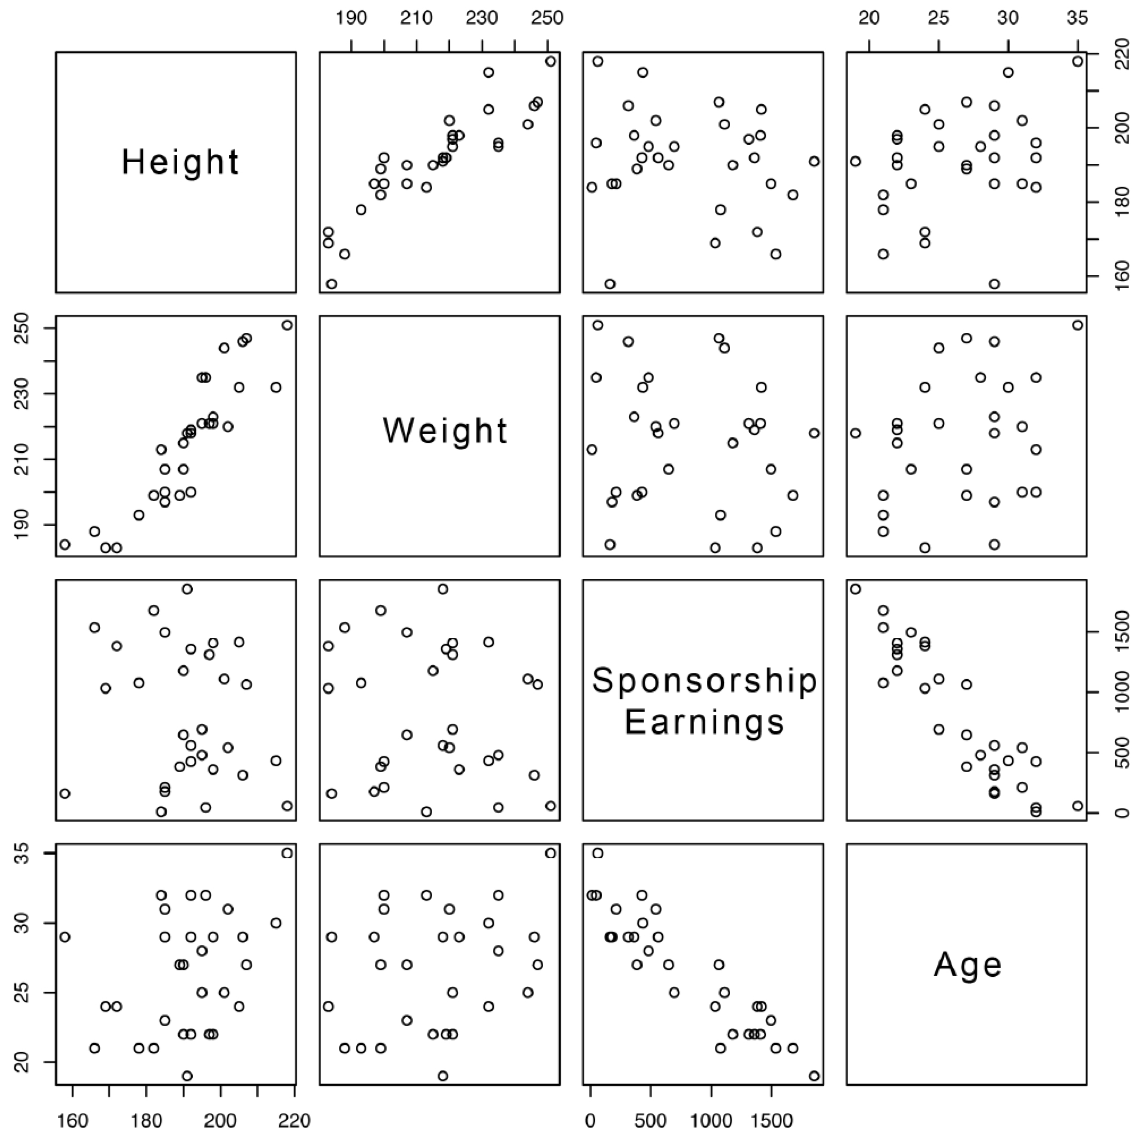
\includegraphics[width=0.7\textwidth]{assets/visualization_and_extraction/feature_relation/splom.png}
  \caption{Scatter plot matrix for four features}
  \label{fig:2_splom}
\end{figure}

Interesting to see in such a SPLOM is the mirror axis in opposite tiles of the matrix which is an absolutely linear line (so absolute correlation, or identity, as would be displayed if a feature would be displayed on a scatter plot compared to itself). This mirroring doesn't change the nature of a correlation. If feature A is positively correlated to feature B, the same goes in the other direction (equivalent for negative correlation).

\subsubsection*{Small multiple bar plots}

Another way to display relations is via a collection of small multiple bar plots. Consider the plots in \ref{fig:2_barplot}

\begin{figure}[H]
  \centering
  \begin{subfigure}{0.8\textwidth}
    \centering
    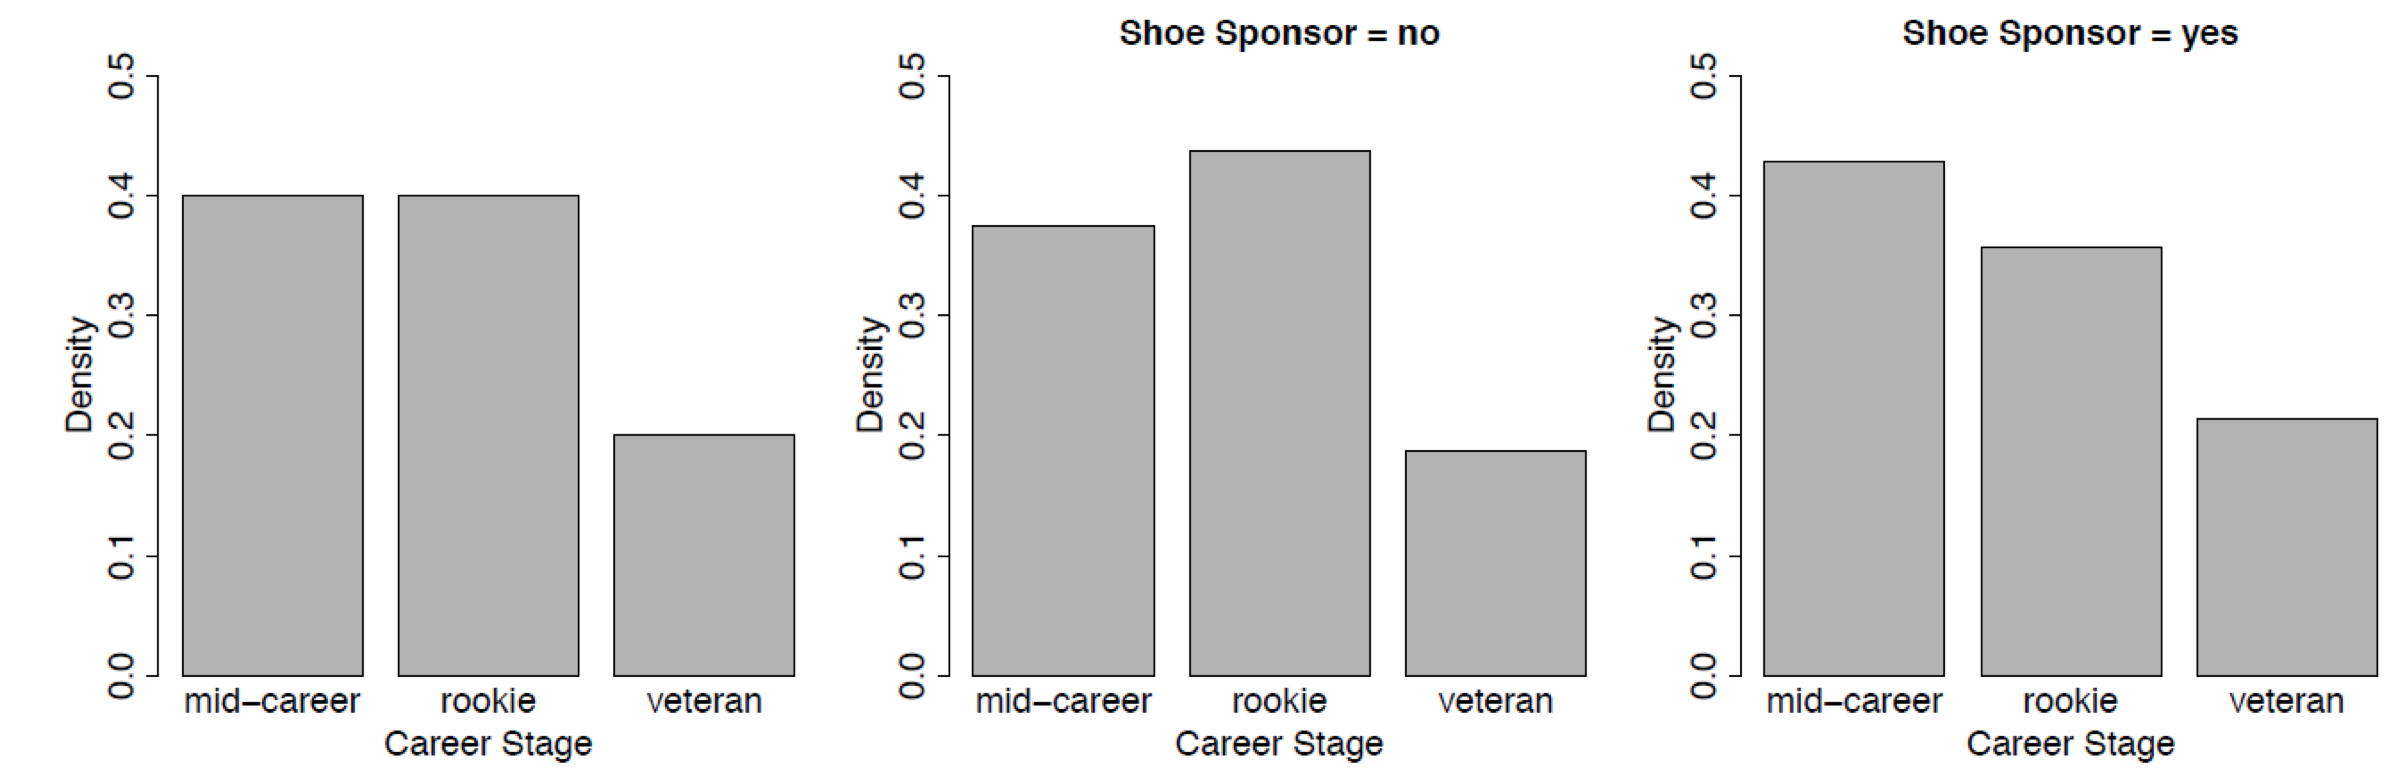
\includegraphics[width=\textwidth]{assets/visualization_and_extraction/feature_relation/bar_no.png}
    \subcaption{No relation}
  \end{subfigure}
  
  \vspace*{0.2cm}

  \begin{subfigure}{0.75\textwidth}
    \centering
    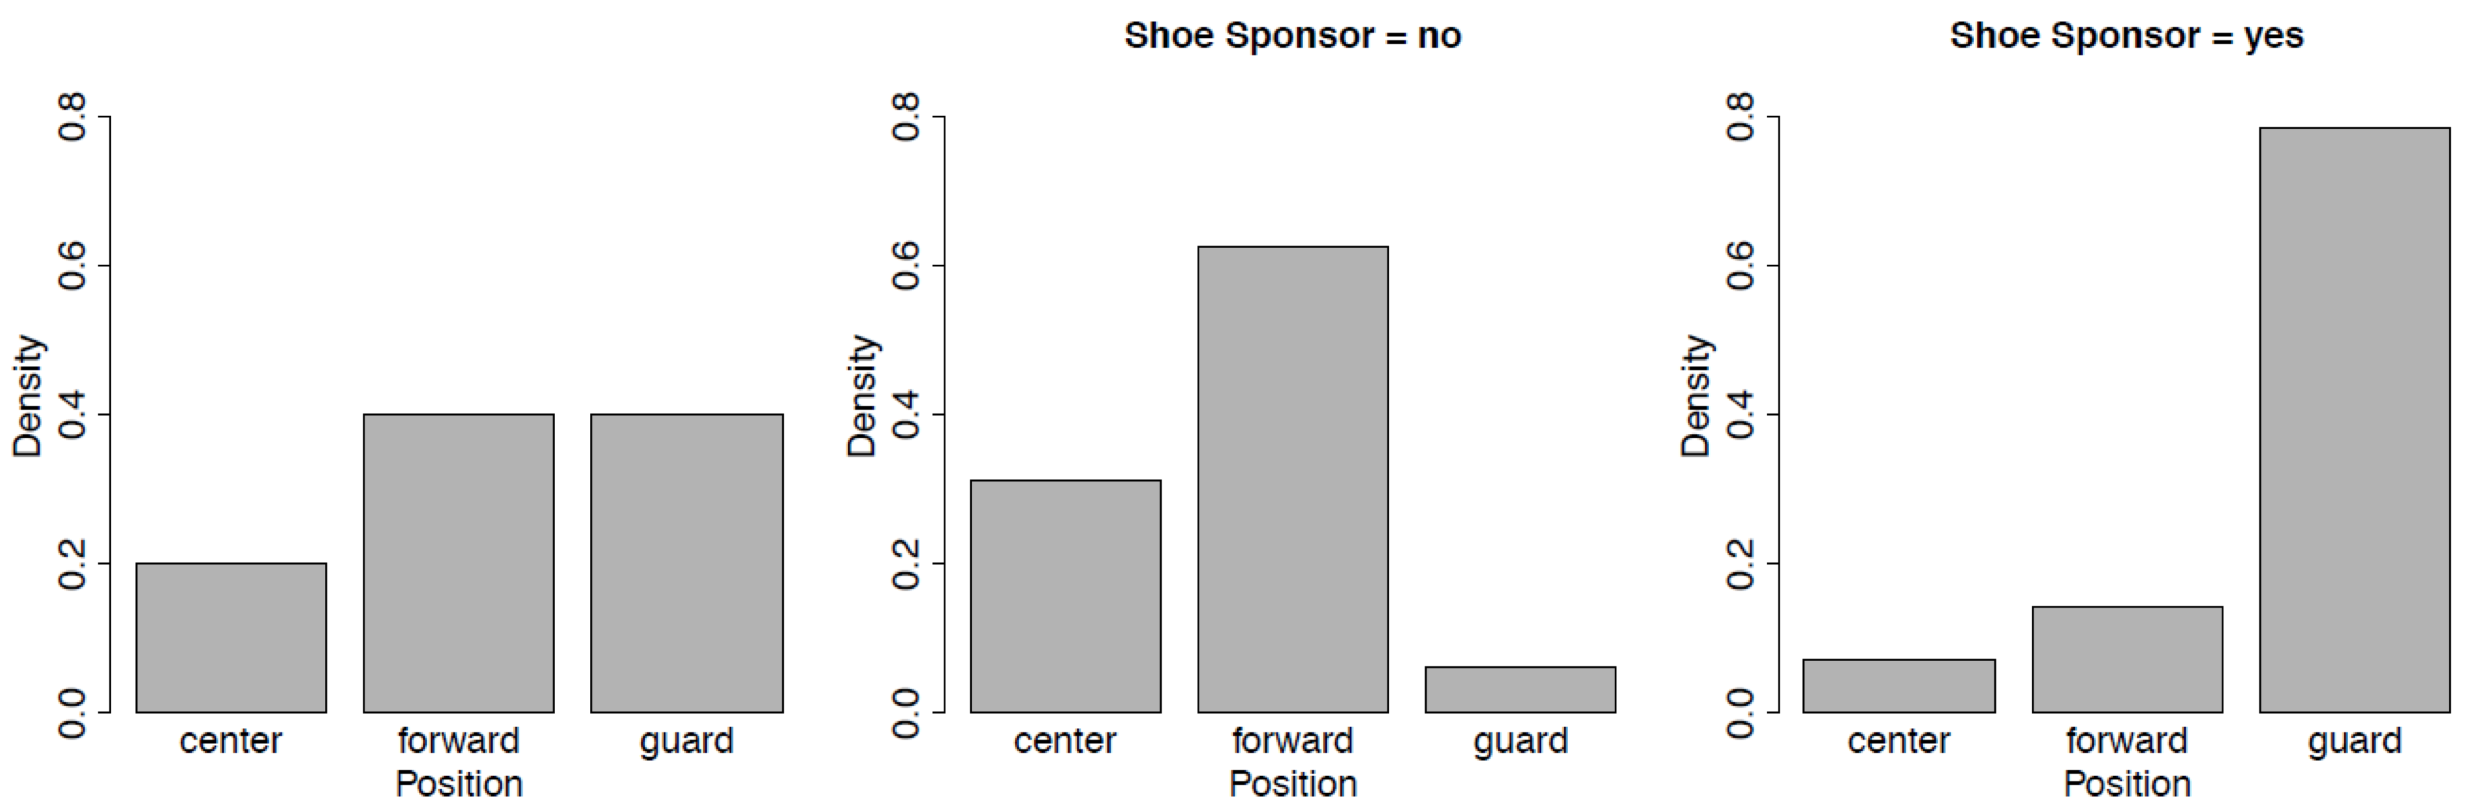
\includegraphics[width=\textwidth]{assets/visualization_and_extraction/feature_relation/bar_strong.png}
    \subcaption{Strong relation}
  \end{subfigure}
  \caption{Collection of (conditioned) bar plots}
  \label{fig:2_barplot}
\end{figure}